
\documentclass[aspectratio=1610]{beamer}

\usepackage[utf8]{inputenc}
\usepackage[T1]{fontenc}
\usepackage{amsmath,amssymb,amsfonts}
\usepackage{hyperref} % before url package otherwise there is a pb
\usepackage{url}

\setbeamertemplate{navigation symbols}{%
    \usebeamerfont{footline}%
    \usebeamercolor[fg]{footline}%
    \hspace{1em}%
    \insertframenumber/\inserttotalframenumber
}
\setbeamercolor{footline}{fg=black}


\usepackage{comment}

\usepackage{algorithmic}
\usepackage[ruled,noline,noend]{algorithm2e}
\algomargin 0pt
\SetAlCapHSkip{0pt}
\DontPrintSemicolon
\SetKw{Continue}{continue}
% fix bug in algorithm2e
\makeatletter
\renewcommand{\@algocf@start}{%
  \@algoskip%
  \begin{lrbox}{\algocf@algobox}%
  \setlength{\algowidth}{\hsize}%
  \vbox\bgroup% save all the algo in a box
  \hbox to\algowidth\bgroup\hbox to \algomargin{\hfill}\vtop\bgroup%
  \ifthenelse{\boolean{algocf@slide}}{\parskip 0.5ex\color{black}}{}%
  % initialization
  \addtolength{\hsize}{-\algomargin}%
  % we don't want our algorithm lines numbered, so let's ditch that right
  % space.
  % \addtolength{\hsize}{-1.5em}% 1.5em to let space for line numbering
  \let\@mathsemicolon=\;\def\;{\ifmmode\@mathsemicolon\else\@endalgoln\fi}%
  \raggedright%
  \AlFnt{}%
  \ifthenelse{\boolean{algocf@slide}}{\IncMargin{\skipalgocfslide}}{}%
  \@algoinsideskip%
%   \let\@emathdisplay=\]\def\]{\algocf@endline\@emathdisplay\nl}%
}%
\makeatother

\usepackage{tikz}
\usetikzlibrary{calc, positioning, arrows.meta}
\usetikzlibrary{shapes.geometric} % for ellipse
\usetikzlibrary{arrows}
\usetikzlibrary{positioning}
\tikzset{
  state/.style={
    rectangle,
    rounded corners,
    draw=black, thick,
    minimum height=2em,
    inner sep=2pt,
    text centered,
  },
}
\usetikzlibrary{tikzmark}
\usepackage{pgfplots}

\usepackage{multirow}
\usepackage{multicol}

\newcommand{\NN}{\ensuremath{\mathbb N}}
\newcommand{\ZZ}{\ensuremath{\mathbb Z}}
\newcommand{\QQ}{\ensuremath{\mathbb{Q}}}
\newcommand{\RR}{\ensuremath{\mathbb{R}}}
\newcommand{\CC}{\ensuremath{\mathbb{C}}}
\newcommand{\K}{\ensuremath{\mathbb{K}}}
\newcommand{\PP}{\ensuremath{\mathbb{P}}} % for projective line
\newcommand{\FF}{\ensuremath{\mathbb F}}
\newcommand{\F}{\ensuremath{\mathbb F}}
\newcommand{\GG}{\ensuremath{\mathbb G}}
\newcommand{\G}{\ensuremath{\mathbb G}}
\newcommand{\GT}{\ensuremath{\mathbb G_{\text{T}}}}
\newcommand{\Fp}{\F_p}
\newcommand{\cO}{\ensuremath{\mathcal O}}
\newcommand{\cF}{\ensuremath{\mathcal F}}
\DeclareMathOperator{\Norm}{Norm}
\DeclareMathOperator{\ord}{ord}
\DeclareMathOperator{\disc}{Disc}
\DeclareMathOperator{\coeff}{Coeff}
\DeclareMathOperator{\cont}{cont}
\DeclareMathOperator{\reslt}{Res}
\DeclareMathOperator{\Reslt}{Res}
\DeclareMathOperator{\Res}{Res}
\DeclareMathOperator{\val}{val}
\DeclareMathOperator{\GF}{GF}
\DeclareMathOperator{\aut}{aut}
\DeclareMathOperator{\End}{End}
\DeclareMathOperator{\lc}{lc} % for leading coefficient
\DeclareMathOperator{\Id}{Id} % for Identity
\DeclareMathOperator{\Div}{div}
\newcommand{\BLS}{\mbox{BLS}}

\usepackage{fontawesome}

\date{November 19th, 2025 -- Buenos Aires, DevConnect}
\title{Kohaku Hardware Signer: First Post-Quantum Secure Element Implementation}
\author{\textbf{Simon Masson}, Renaud Dubois\\
ZKNox\\
\includegraphics[height=4em]{zknox.png}\\
Account Abstraction Hub}
\begin{document}
\begin{frame}
  \maketitle
\end{frame}

\begin{frame}{ZKNOX team}
  \begin{minipage}{.65\linewidth}
   \begin{tabular}{rl}
      \multirow{4}{*}{\includegraphics[width=2cm]{NB.jpeg}} & \textbf{Nicolas Bacca}\\
                               & \small{$20^+$ years experience ($10^+$y web3)}\\
                               & Security and hardware specialist\\
                               & \small{Prev.~Ledger cofounder/CTO}\\
                               & \\
      \multirow{4}{*}{\includegraphics[width=2cm]{RD.jpeg}} & \textbf{Renaud Dubois}\\
                               & \small{$20^+$ years experience ($3^+$y web3)}\\
                               & Cryptographer\\
                               & \small{Prev.~Ledger, Thales}\\
                               & \\
      \multirow{4}{*}{\includegraphics[width=2cm]{SM.jpg}} & \textbf{Simon Masson}\\
                               & \small{$8^+$ years experience ($4^+$y web3)}\\
                               & Cryptographer\\
                               & \small{Prev.~Heliax, Thales}\\
  \end{tabular}
\end{minipage}\pause
\begin{minipage}{.33\linewidth}
   Expertise and innovation to every challenge on the whole security chain:
   \begin{itemize}
   \item user end\\ (secure enclaves, hardware wallets),
   \item back end\\ (TEE, HSMs),
   \item on-chain\\ (smart contracts).
   \end{itemize}

  \pause
 
  \vspace{1em}

  \href{https://zknox.eth.limo/}{\texttt{https://zknox.eth.limo/}}

  \vspace{1em}

  \href{https://github.com/zknoxhq/}{\texttt{https://github.com/zknoxhq/}}

\end{minipage}
\end{frame}

% \begin{frame}{Alice sends 1.0 ETH to Bob (signed transaction)}

%   \begin{tikzpicture}[every node/.style={font=\small}, node distance=2.0cm]
%     % Wallet style
%     \tikzset{wallet/.style={rectangle,draw,rounded corners=4pt,minimum width=3.4cm,minimum height=1.0cm,align=center}}
%     \node[wallet] (alice) {Alice\\\texttt{0xAa...1}};
%     \node[wallet, right=5.5cm of alice] (bob) {Bob\\\texttt{0xBb...2}};

%     % Arrow
%     \draw[->, line width=1.2pt] (alice.east) -- node[above,midway] {\small 1.0 ETH \\ \small txHash: \texttt{0xabc\dots123}} (bob.west);

%     % Signature bubble
%     \node[draw,rounded corners=4pt,right=0.0cm of alice, yshift=-2.0cm, minimum width=6.5cm, minimum height=1.6cm, font=\footnotesize, align=left] (sigbox) {
%       \textbf{Signed transaction (ECDSA / secp256k1)}\\[2pt]
%       Signature components: \\
%       \quad $r$ = \texttt{0x7f3a...e9a} \\
%       \quad $s$ = \texttt{0x5c2b...4d1} \\
%       \quad $v$ = \texttt{0x1b} (27) or 28
%     };

%     % nonce/gas label
%     \node[below=0.8cm of alice, align=left,font=\small] (meta) {
%       \textbf{Transaction metadata}\\
%       \quad nonce: 5 \quad gasPrice: 50 Gwei \quad gasLimit: 21000
%     };

%   \end{tikzpicture}
% \end{frame}





\begin{frame}{Account Abstraction}
  \begin{center}
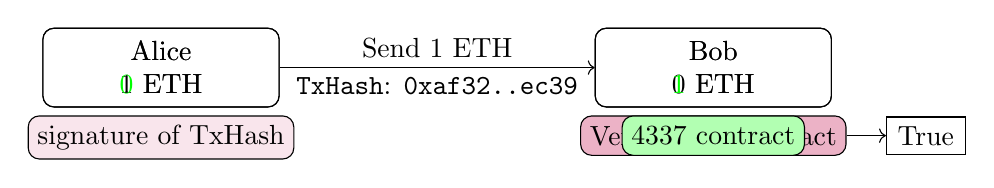
\begin{tikzpicture}[
  note/.style={draw, rounded corners, minimum width=3cm, minimum height=1cm, align=center},
  sigbox/.style={draw, fill=purple!10, rounded corners, minimum width=2cm, minimum height=.5cm, align=center},
  verifbox/.style={draw, fill=purple!30, rounded corners, minimum width=2cm, minimum height=.5cm, align=center},
  4337box/.style={draw, fill=green!30, rounded corners, minimum width=2cm, minimum height=.5cm, align=center},
  boolbox/.style={draw, minimum width=1cm, minimum height=.25cm, align=center},
  arrow/.style={thick, ->, >=Stealth}
]

% Notes
\onslide<1-4>{\node[note] (alice) {Alice \\ 1 ETH};}
\onslide<1-4>{\node[note, right=4cm of alice] (bob) {Bob \\ 0 ETH};}
\onslide<5->{\node[note] (alice) {Alice \\ \textcolor{green}{0} ETH};}
\onslide<5->{\node[note, right=4cm of alice] (bob) {Bob \\ \textcolor{green}{1} ETH};}
\onslide<2->{\draw[->](alice) -- (bob) node[midway, above]{Send 1 ETH} node[midway,below]{\texttt{TxHash}: \texttt{0xaf32..ec39}};}
\onslide<3->{\node[sigbox, below=0.1cm of alice] (sig) {signature of TxHash};}
\onslide<4-5>{\node[verifbox, below=0.1cm of bob] (verif) {Verification contract};}
\onslide<5->{\node[boolbox, right=0.5cm of verif] (bool) {True};}
\onslide<5->{\draw[->](verif) --  (bool);}
\onslide<6->{\node[4337box, below=0.1cm of bob] (verif) {4337 contract};}
\end{tikzpicture}
\end{center}

  \onslide<7->{Execution layer: ECDSA signature (not resistant to quantum attacks)}
   
  \onslide<8->{Account abstraction (4337): enables custom signature.}

  \onslide<9->{This work: 
  \begin{itemize}
    \item smart account with hybrid ECDSA+MLDSA verification,
    \item same user experience, but hardware and post-quantum security.
  \end{itemize}}

\end{frame}

\begin{frame}{Post-quantum signature candidates}

  \begin{center}
    \begin{tabular}{|l|c|c|c|}
      \hline
      Standard & \textbf{FN-DSA} & \textbf{ML-DSA} & \textbf{SLH-DSA}\\
      Name & Falcon & Dilithium & Sphincs\\
      FIPS & 203 & 204 & 205\\
      Family & Lattice & Lattice & Hash\\
      \hline 
      Signature & \onslide<2->{\textcolor{green}{666B}} & \onslide<2->{\textcolor{orange}{2420B}} & \onslide<2->{\textcolor{red}{7856B}}\\
      \hline 
      Public key & \onslide<2->{897B} & \onslide<2->{\textcolor{orange}{1312B}} & \onslide<2->{32B}\\
      \hline 
      Signer & \onslide<3->{\textcolor{orange}{floating point}, high RAM} & \onslide<3->{Simple} & \onslide<3->{Very slow}\\
      \hline
      Verifier & \onslide<3->{\textcolor{green}{separation} hash-core, efficient} & \onslide<3->{Simple} & \onslide<3->{\textcolor{red}{Very slow}}\\
      \hline 
    \end{tabular}
  \end{center}

  \onslide<4->{We implement ML-DSA (Dilithium) following EIP 8051}
\end{frame}

\begin{frame}{EIP 8051}
  Two precompiles:
  \begin{itemize}
    \item ML-DSA-NIST: using the hash function SHAKE256 (compliant to NIST)
    \item ML-DSA-ETH: using the hash function KECCAK256 (efficient in Ethereum contracts)
  \end{itemize}
  \pause 
  Public key is expanded during verification:
  \begin{center}
    \begin{tikzpicture}[
      pk/.style={draw, rounded corners, minimum width=1cm, minimum height=.5cm, align=center},
      pkexp/.style={draw, fill=purple!10, rounded corners, minimum width=2cm, minimum height=.5cm, align=center},
      % verifbox/.style={draw, fill=purple!30, rounded corners, minimum width=2cm, minimum height=.5cm, align=center},
      % 4337box/.style={draw, fill=green!30, rounded corners, minimum width=2cm, minimum height=.5cm, align=center},
      % boolbox/.style={draw, minimum width=1cm, minimum height=.25cm, align=center},
      % arrow/.style={thick, ->, >=Stealth}
    ]

    % Notes
    \onslide<1->{\node[pk] (pk) {Public key\\1312B};}
    \onslide<2->{\node[pk, right=4cm of alice] (pkexp) {Expanded public key ($\mathbb F_q^{4\times 4}, bytes, \mathbb F_q^4$)\\\textbf{20512B}};}
    \onslide<2->{\draw[->](pk) -- (pkexp) node[midway, above]{using hash};}
    \end{tikzpicture}
  \end{center}


  \onslide<3->{Public key provided in expanded form to save hashes.}
  
  \onslide<4->{Verifier cost: \textbf{5} calls to hash (SHAKE256 or KECCAK256) and \textbf{9} NTTs.}

\end{frame}

\begin{frame}{Hardware implementation}
  \begin{itemize}[<+->]
    \item Start from NIST FIPS 204 reference code
    \begin{center}
      \includegraphics[width=5cm]{nist-github.png}
    \end{center}
    \item Adaptations for low ram constraints:
    \begin{center}
      \includegraphics[scale=.25]{keystone.png}
      \includegraphics[scale=.25]{trezor.png}
      \includegraphics[scale=.25]{flex.png}
    \end{center}
    \item Ledger RAM $\leq 50$kB $\Rightarrow$ implem.~as in ia.cr/2022/323 (thanks to \texttt{dop-amin})
    \item Entire computation in the Secure Element (the secret never leaves the enclave)
    \item Provide two signers for the two precompiles:
    \begin{itemize}
      \item MLDSA (SHAKE256 using NIST code) signing in 700ms,
      \item MLDSA-ETH (Keccak256 BOLOS calls) signing slower (BOLOS communication).
    \end{itemize}
    \item Implementation tricks:
    \begin{itemize}
      \item Recomputation of keygen to save RAM access,
      \item Tweaked BIP32 to derive unique secret per hardware
      \item Public key (resp.~signature) fetching requires 6 APDUs (resp.~10 APDUs) to get 255B chunks
    \end{itemize}
    \item Soon on other HW...
  \end{itemize}
\end{frame}

% demonstration
\begin{frame}{Demonstration}
  Let's see how it works in practice

    \vspace{2cm}

  \begin{center}
  soon in

  \includegraphics[width=8cm]{kohaku.png}
  \end{center}
\end{frame}

\begin{frame}{Hybrid 4337}
  \begin{itemize}[<+->]
    \item MLDSA Expanded public key stored on-chain (20512B) per user
    \item Hybrid contract:
    \begin{enumerate}
      \item Fetches the MLDSA public key
      \item Verifies the Post-Quantum signature
      \item Fetches the ECDSA public key (or Ethereum address)
      \item Verifies the ECDSA signature using \texttt{ecrecover}
      \item Accepts only if \textbf{both} signatures are valid.
    \end{enumerate}
  \end{itemize}

    \begin{center}
      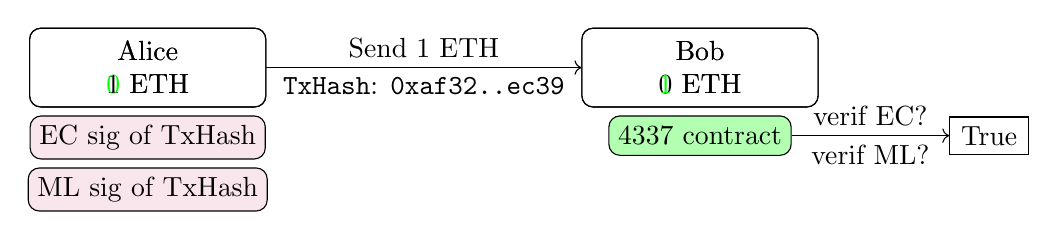
\begin{tikzpicture}[
        note/.style={draw, rounded corners, minimum width=3cm, minimum height=1cm, align=center},
        sigbox/.style={draw, fill=purple!10, rounded corners, minimum width=2cm, minimum height=.5cm, align=center},
        sigbox2/.style={draw, fill=purple!10, rounded corners, minimum width=2cm, minimum height=.5cm, align=center},
        verifbox/.style={draw, fill=purple!30, rounded corners, minimum width=2cm, minimum height=.5cm, align=center},
        4337box/.style={draw, fill=green!30, rounded corners, minimum width=2cm, minimum height=.5cm, align=center},
        boolbox/.style={draw, minimum width=1cm, minimum height=.25cm, align=center},
        arrow/.style={thick, ->, >=Stealth}
      ]

      % Notes
      \onslide<8-9>{
        \node[note] (alice) {Alice \\ 1 ETH};
        \node[note, right=4cm of alice] (bob) {Bob \\ 0 ETH};
      }
      \onslide<10->{
        \node[note] (alice) {Alice \\ \textcolor{green}{0} ETH};
        \node[note, right=4cm of alice] (bob) {Bob \\ \textcolor{green}{1} ETH};
      }
      \onslide<8->{
        \draw[->](alice) -- (bob) node[midway, above]{Send 1 ETH} node[midway,below]{\texttt{TxHash}: \texttt{0xaf32..ec39}};
      }
      \onslide<9->{
        \node[sigbox, below=0.1cm of alice] (sig) {EC sig of TxHash};
        \node[sigbox2, below=0.1cm of sig] (sigpq) {ML sig of TxHash};
      }
      \onslide<10->{
        \node[4337box, below=0.1cm of bob] (verif) {4337 contract};
        \node[boolbox, right=2cm of verif] (bool) {True};
        \draw[->](verif) --  (bool) node[midway, above]{verif EC?} node [midway, below]{verif ML?};
      }
    \end{tikzpicture}
  \end{center}
  \onslide<11->{
    Thanks to Alex and Shahaf from 4337 team for the integration help :-)
  }
\end{frame}

\begin{frame}{Conclusion and perspectives}
 \begin{itemize}[<+->]
  \item[$\checkmark$] Hardware implementation of MLDSA and MLDSAETH,
  \item[$\checkmark$] Hybrid 4337 account with ECDSA and MLDSA,
  \item [$\Box$] BIP32 compliant secret derivation,
  \item [$\Box$] Universal Ethereum app enables FN-DSA and ML-DSA on other HW,
  \item [$\Box$] More comparisons with FN-DSA,
  \item [$\Box$] Experiments on L2 possible but gas is expensive.
  \end{itemize}
  \begin{flushright}
  \onslide<7>{Thank you for your attention.}
  \end{flushright}
\end{frame}


\end{document}
